\section{Ethernet}
\subsection{Begriffe}

\subsubsection{Topologien}
\begin{center}
	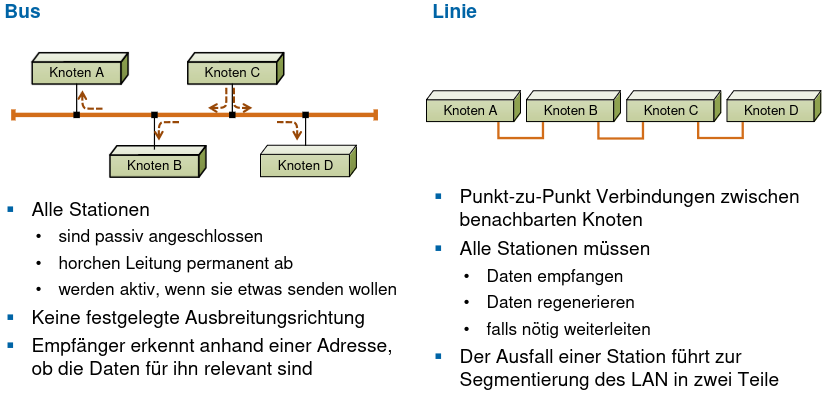
\includegraphics[width=0.8\linewidth]{topo-bus-linie}

	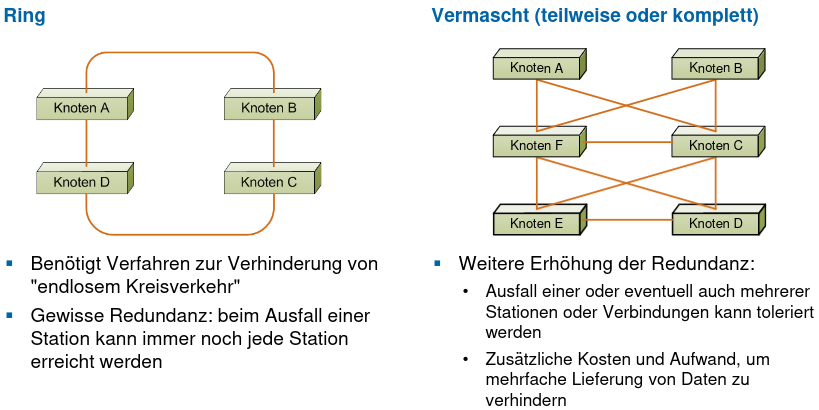
\includegraphics[width=0.8\linewidth]{topo-ring-mesh}

	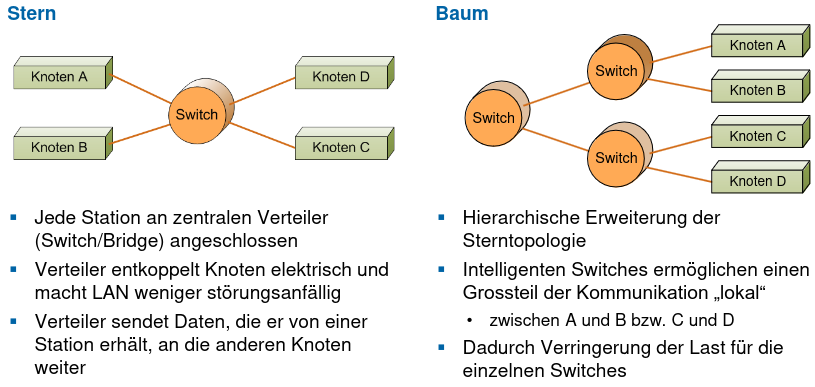
\includegraphics[width=0.8\linewidth]{topo-stern-baum}
\end{center}

\subsubsection{Übertragungsarten}
Immer nur ein Sender! Anzahl empfänger unterscheidet sich

\begin{description}
	\item[Unicast] Genau 1 klar definierter Empfänger, Frame trägt dessen Adresse
	\item[Multicast] Gruppe von Empfängern, Frame trägt Adresse dieser Gruppe
	\item[Broadcast] An alle Knoten im LAN, Frame trägt Broadcast-Adresse
\end{description}

\subsubsection{MAC-Adresse}

Erste drei Byte Hersteller + Individual/Group \& Universally/Locally bits,
die letzen drei Bytes Laufnummer durch Hersteller

\begin{center}
	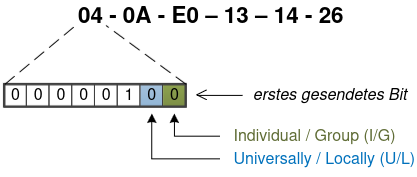
\includegraphics[width=0.8\linewidth, height=15mm]{mac-ig-ul}
\end{center}




\subsection{Ethernet Frame}
\begin{itemize}
	\item Bit Synchronisation durch Präamble, Bytes \& Frames durch Start
	      Frame Delimiter (SFD = 1010'1011)
	\item Frame-Länge 64 .. 1518 Byte (ohne Präable und SFD)
	\item Bytes nacheinander übertagen, pro Byte \textcolor{red}{LSB} zuerst
	\item Zahlenwerte (Length/Type/...) höchstwertiges Byte zuerst gesendet
	      (Network Byte Order)
\end{itemize}
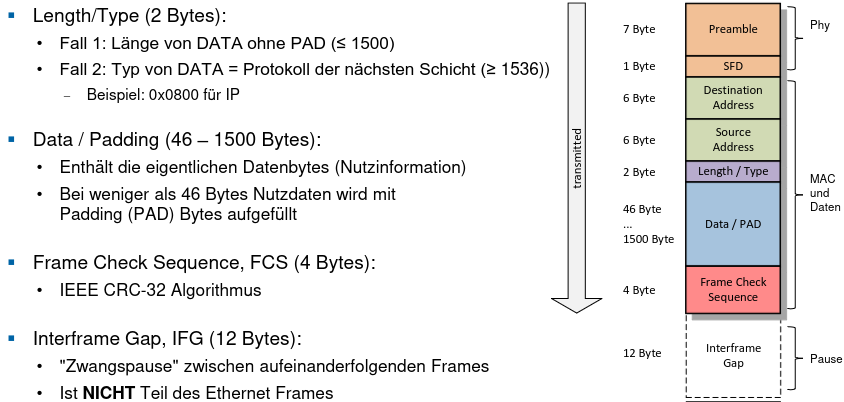
\includegraphics[width=\linewidth]{eth-frame-fields}

Die FCS wird mit IEEE CRC-32 berechnet. Die Hamming-Distanz ist Abhängig von der
Frame-Länge: 6 bis 226, danach 5 bis 2974 (Ethernet Limit = 1518)

\subsubsection{Kennzahlen zu Ethernet}
\begin{description}
	\item[Overhead] 18 Bytes aus DA,SA,L/T,FCS
	\item[Frame-Size] 64 bis 1518 Bytes
	\item[Sendedauer] $T_{frame} =
			\frac{N_{bit} = (\text{FrameSize} + 8) * 8}{\text{Bitrate}}$
	\item[Dauer der Leitungsbelegung] $T_{leitung}
			= \frac{N_{bit} + 96}{\text{Bitrate}}$
\end{description}





\subsection{Network Gear}

Kreiren eine Broadcast Domain / LAN, Endgeräte merken davon nichts (transparent)
sondern sprechen aus ihrer sicht direkt den Empfänger an.

\begin{description}
	\item[Repeater/Hubs] verstärkt Signal von einem Port und leitet sie weiter
		auf allen anderen
	\item[Bridge/Switch] lernt Adressen, leitet Daten weiter an
		die richtigen ports (Filtering Database)
\end{description}



\subsection{VLAN (802.1Q)}

Repräsentiert eigene, virtuelle Broadcastdomain. \\
Auf einem Switch kann jedem Port nur eine VLAN-ID gegeben werden, da die Zuordnung
erst am Switch selbst passiert (muss konfiguriert werden, ''managed switch'').

Bei VLAN gibt es 2 verschiedene Arten von Links (Verbindung zwischen Geräten).
\begin{description}
	\item[Access Links] nur einem VLAN zugehörig
	\item[Trunk Links] oft zwischen Switches, gesendete Frames können mehreren VLANs
		angehören $\rightarrow$ Frames müssen vom Switch getagged werden
\end{description}

\begin{center}
	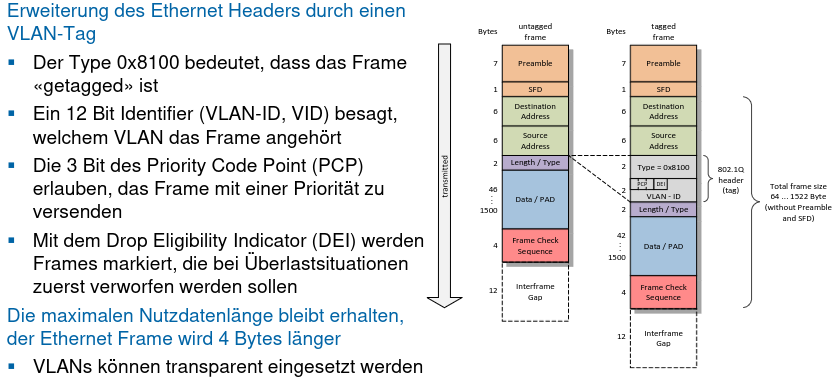
\includegraphics[width=0.9\linewidth]{vlan-frame}
\end{center}

PCP: höhere Prio kann tiefere überholen in der Bridge


\subsection{(Rapid) Spanning Tree}

Ziel: Alle Segmente in einer loop-freien Topologie verbinden \\
Idee: \begin{enumerate}
	\item willkürliche aber eindeutige Root-Bridge wählen
	\item von Root aus Baum aufbauen
	\item redundante Pfade sperren
\end{enumerate}

Algorithmus: \\
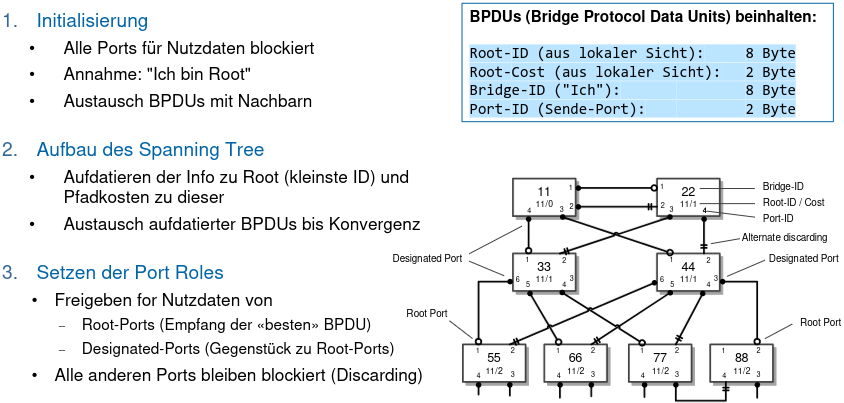
\includegraphics[width=0.9\linewidth]{spanning-tree-algo}

Das normale STP konvergiert \& reagiert sehr langsam, die Rapid Variante RSTP
ist vom Grundkonzept identisch aber reagiert schneller auf Topologieänderungen ($\sim$500ms)



\subsection{Evolution von Ethernet}

Bezeichnung(802.3): [Bitrate in Mbit/s] BASE/BROAD-[Art/Codierung]
\small{Bemerkung: früher statt Art/Codierung die max. Segmentlänge in 100m}

\begin{multicols*}{2}
	Beispiele von relevanten in diesem Rahmen
	\begin{itemize}
		\item 10 Mb/s: 10Base-T
		\item 100 Mb/s: 100Base-TX
		\item 1000 Mb/s: 1000Base-T
		\item[\vspace{\fill}]
	\end{itemize}
	\columnbreak
	Codierungsarten:
	\begin{description}
		\item[T, TX, T1] Twisted Pair
		\item[SR, DR, LR] optisch
		\item[C] Twinax
		\item[K] Backplane
	\end{description}
\end{multicols*}

\subsubsection{Autonegotiation}

Für Rückwärtskompatibilität, damit Sender \& Empfänger wissen was möglich ist. \\
Umgesetzt mittels Fast Link Pulses \textbf{FLP} (seit 100BASE-TX) zwischen den regulären Normal Link
Pulses NLP(10BASE-T).

\subsubsection{100BASE-TX}
\begin{description}
	\item[Coderiung] NRZI + umwandeln von 4 Bits in 5-Bit PCS (4B5B)
	\item[Start-of-Stream] ähnlich zu 10BASE-T Preamble, bestimmte PCS Zeichen J/K
	\item[End-of-Stream] markiert Ende des Frame, bestimmte PCS Zeichen T/R
	\item[IDLE] NEU: die Leitung wird ununterbrochen mit IDLE gefüllt falls keine
		Nutzdaten, PCS Zeichen I
\end{description}


\subsubsection{1000BASE-T}
\begin{itemize}
	\item 5-wertiger Leitungscode PAM-5
	\item Vollduplex: Alle 4 Aderpaare in beide Richtungen dank Gabelschaltung
	\item Next-Page bei FLP
\end{itemize}


\subsubsection{10GBASE-T}
\begin{itemize}
	\item 16-wertiger Leitungscode PAM-16
	\item Effizientere Verteilung der Bits auf Adernpaare
	\item forward error correction
	\item neuer Stecker ab CAT7: GG45
\end{itemize}



